\documentclass[11pt,a4paper]{article}

\usepackage[T1]{fontenc}
\usepackage{lmodern}
\usepackage[margin=2.2cm]{geometry}
\usepackage{booktabs}
\usepackage{longtable}
\usepackage{tabularx}
\usepackage{array}
\usepackage{caption}
\usepackage{subcaption}
\usepackage{float}
\usepackage{graphicx}
\usepackage[hidelinks]{hyperref}
\usepackage{microtype}

\setlength{\parindent}{0pt}
\setlength{\parskip}{0.6em}
\setlength{\emergencystretch}{2em}
\renewcommand{\arraystretch}{1.15}
\captionsetup{labelsep=period}
\captionsetup[subfigure]{
    font=scriptsize,
    justification=raggedright,
    singlelinecheck=false,
    skip=2pt
}

\newcolumntype{L}[1]{>{\raggedright\arraybackslash}p{#1}}
\newcolumntype{Y}{>{\raggedright\arraybackslash}X}

\begin{document}

\setcounter{section}{2}

\section{Testing Report}
\label{sectestingreport}

\subsection{Testing Rationale and Objectives}
\label{subsectestingrationale}

The usability test assessed whether the prototype allowed participants to
complete the core tasks without help. It checked each acceptance criterion and
showed where users misunderstood a control, a message, or a change in system
state. The team compared observed behaviour with completion data and participant
comments. The findings were then used to decide which requirements and screens
needed revision before the next iteration.

\subsection{Participants and Method}
\label{subsectestingmethod}

\subsubsection{Participants}

Five purposively selected participants covered student and working-adult
contexts, different rental and shared-living experience, colour-accessibility,
mobile-first use and different English-language backgrounds
(Table~\ref{tabiterationoneparticipants}). They were recruited through the
project team network and screened for these contexts. Participation was
voluntary and unpaid, and consent was obtained before each session.

\begin{table}[H]
    \centering
    \small
    \caption{Iteration 1 participant profile.}
    \begin{tabularx}{\textwidth}{@{}L{1.5cm}L{3.8cm}Y@{}}
        \toprule
        ID & User group & Relevant context\\
        \midrule
        User A &
        UNSW student &
        High cleanliness standards and interest in household hygiene.\\
        User B &
        Domestic UNSW student &
        Colour vision deficiency.\\
        User C &
        Employed UNSW graduate living in a shared apartment &
        English is not the first language.\\
        User D &
        Newly arrived international student &
        No Australian rental experience; primarily uses a mobile phone.\\
        User E &
        Young professional &
        More than three years of shared-living experience; previously searched
        for housemates and established common-area rules.\\
        \bottomrule
    \end{tabularx}
    \label{tabiterationoneparticipants}
\end{table}

\subsubsection{Procedure and Measures}

Five participants tested version 1.3 of the HTML prototype across one tablet,
two laptops and two mobile devices between 25 and 27 July 2026. The allocation
is shown in Table~\ref{tabiterationonedevices}.

\begin{table}[H]
    \centering
    \small
    \caption{Iteration 1 participant device allocation.}
    \begin{tabularx}{\textwidth}{@{}L{1.6cm}L{2.4cm}L{4.1cm}L{2.5cm}Y@{}}
        \toprule
        User & Date & Device & Browser & Viewport\\
        \midrule
        User A & 25 July 2026 & iPad tenth generation & Safari & 1180 by 820\\
        User B & 25 July 2026 & MacBook Air M2 & Chrome & 1440 by 900\\
        User C & 26 July 2026 & Dell Inspiron 14 & Microsoft Edge & 1366 by 768\\
        User D & 26 July 2026 & iPhone 13 & Safari & 390 by 844\\
        User E & 27 July 2026 & Samsung Galaxy S22 & Chrome & 360 by 800\\
        \bottomrule
    \end{tabularx}
    \label{tabiterationonedevices}
\end{table}

Each moderated session used the same seeded account and task state.
Participants attempted T1 to T5 while thinking aloud. The facilitator gave a
hint only after a participant was unable to continue for 30 seconds. The
observer recorded final-state completion, time, errors, assistance and
interpretation of feedback. Wrong controls, pages or unsupported actions
counted as errors; assisted completions were not independent. Only task means
were available, so individual time-threshold compliance could not be confirmed
and will be captured in Iteration 2.

\subsection{Iteration 1 Testing}
\label{subseciterationone}

\subsubsection{Test Plan and Acceptance Criteria}

Iteration 1 retained the five tasks and acceptance-criteria identifiers from
Part 2, but expanded coverage from the original mobile viewport to tablet,
laptop and mobile contexts. Task outcome and acceptance-criteria status were
assessed separately. A task was \textit{Completed} only when at least four of
five participants independently met every behaviour, interpretation and time
condition in its measurable threshold. It was \textit{Partially completed}
when participants reached some or all of the workflow but one or more
conditions were failed or not separately tested. Each acceptance criterion was
classified as Pass, Partial, Fail or Not separately tested. Partial means that
some required behaviour was demonstrated but the full measurable threshold was
not met; task completion alone did not override a criterion-level result.
AC-US11-01 and AC-US09-01 used seeded, simulated states, so testing assessed
usability rather than production verification or messaging security.

\begin{table}[H]
    \centering
    \footnotesize
    \caption{Iteration 1 test plan and acceptance criteria coverage.}
    \begin{tabularx}{\textwidth}{@{}L{0.7cm}L{2.7cm}L{2.0cm}L{3.3cm}Y@{}}
        \toprule
        Test & User task & Traceability & Acceptance criteria & Measurable success threshold\\
        \midrule
        T1 &
        Narrow properties using combined search criteria &
        US-13; S-01 &
        AC-US13-01 to AC-US13-04 and AC-US13-06 (implemented) &
        At least 4/5 independently complete the filtered search, explain
        affordability, recover from no results and use a custom address within
        three minutes.\\

        T2 &
        Recognise verified housemate profiles &
        US-11; S-02 &
        AC-US11-01 (simulated) and AC-US11-02 (implemented) &
        At least 4/5 independently find the verified-only control, identify its
        cues and explain that verification is not a guarantee within 90 seconds.\\

        T3 &
        Build a profile and use recalculated compatibility &
        US-12; S-03 &
        AC-US12-01, AC-US12-02 and AC-US12-04 to AC-US12-06 (implemented) &
        At least 4/5 independently complete the profile, explain the top match
        and recover from validation and zero-result states within three minutes.\\

        T4 &
        Complete phone verification and message safely &
        US-09; S-04 &
        AC-US09-01 (simulated) and AC-US09-04 (implemented) &
        At least 4/5 independently pass verification and message within three
        minutes; contact details remain blocked with a clear explanation.\\

        T5 &
        Propose, review and activate a house rule &
        US-02, US-10; S-05, S-06 &
        AC-US02-01 to AC-US02-03, AC-US10-01, AC-US10-02 and AC-US10-04
        (implemented) &
        At least 4/5 independently view, propose and activate a rule, including
        language, validation and approval states, within four minutes.\\
        \bottomrule
    \end{tabularx}
    \label{tabiterationoneplan}
\end{table}

\subsubsection{Testing Outcomes}

\begin{table}[H]
    \centering
    \footnotesize
    \caption{Iteration 1 outcome summary.}
    \begin{tabularx}{\textwidth}{@{}L{0.7cm}L{1.4cm}L{3.6cm}Y@{}}
        \toprule
        Test & Task outcome & Quantitative outcome & Acceptance-criteria assessment and consequence\\
        \midrule
        T1 & Partially completed &
        5/5 reached the final state; 4/5 independently; mean 2 min 8 sec;
        2 errors; 1 assisted &
        AC-US13-01 to AC-US13-03: Pass. AC-US13-04: Fail because participants
        did not reliably understand how to recover from the empty state.
        AC-US13-06: Not separately tested. Individual compliance with the
        three-minute limit was also not recorded. Make the recovery action
        more prominent and explicit.\\
        T2 & Partially completed &
        5/5 reached the final state independently; mean 1 min 2 sec;
        1 error; no assistance &
        Simulated AC-US11-01: Pass. Implemented AC-US11-02: Pass. Individual
        compliance with the 90-second limit was not recorded, so the composite
        task threshold was not fully verified. Two users found the explanation
        too small; enlarge it and retain non-colour cues.\\
        T3 & Partially completed &
        4/5 reached the final state; 3/5 independently; mean 2 min 44 sec;
        3 errors; 1 assisted &
        AC-US12-01: Pass. AC-US12-02: Partial because the score source and
        limitations were not explained accurately enough. AC-US12-04 to
        AC-US12-06: Not separately tested. Enlarge the factor explanation and
        show why the score changed.\\
        T4 & Partially completed &
        5/5 reached the final state; 4/5 independently; mean 2 min 18 sec;
        2 errors; 1 assisted &
        Simulated AC-US09-01: Pass. AC-US09-04: Fail. Contact details were
        blocked, but the criterion's clear explanation and safe next step were
        not understood. Link the warning to the contact-sharing action.\\
        T5 & Partially completed &
        4/5 reached the final state; 2/5 independently; mean 3 min 11 sec;
        4 errors; 2 assisted &
        AC-US02-01: Not separately tested. AC-US02-02: Pass.
        AC-US02-03: Not separately tested. AC-US10-01: Pass.
        AC-US10-02: Fail because participants could not reliably connect
        approval progress with activation. AC-US10-04: Not separately tested.
        Combine and emphasise approval and activation status.\\
        \bottomrule
    \end{tabularx}
    \label{tabiterationoneoutcomes}
\end{table}

All five reached the final state in T1, T2 and T4, but task-level completion
did not establish that every included acceptance criterion had passed. T2
provided the strongest result because it required no assistance, while T3 and
T5 had the lowest independent completion and most errors. Problems clustered
around post-action feedback: empty-search recovery, score meaning, contact
blocking and rule approval. Iteration 2 will keep participant-level times and
separate results for every criterion.

\subsubsection{User Feedback}

Table~\ref{tabparticipantfindings} reports the seven accepted
participant-level findings. Device and viewport allocations are given in
Table~\ref{tabiterationonedevices}. The statements paraphrase observation
notes rather than claiming verbatim participant quotations.

{\footnotesize
\begin{longtable}{@{}L{1.2cm}L{0.8cm}L{7.0cm}L{4.8cm}@{}}
    \caption{Participant-level accessibility and device-specific findings.}
    \label{tabparticipantfindings}\\
    \toprule
    User & Task & Observed issue & Effect on task\\
    \midrule
    \endfirsthead
    \caption[]{Participant-level accessibility and device-specific findings
    (continued).}\\
    \toprule
    User & Task & Observed issue & Effect on task\\
    \midrule
    \endhead
    \midrule
    \multicolumn{4}{r}{Continued on next page}\\
    \endfoot
    \bottomrule
    \endlastfoot

    A & T5 &
    Keyboard focus moved outside the Create roster dialog. Escape did not
    close it, and focus was not returned to the opening control after closing. &
    The participant lost the interaction context and required assistance.\\

    B & T2 &
    The Discover tabs did not respond to the arrow keys. Their selected state
    also relied mainly on colour and a thin underline. &
    The participant completed the task with a pointer, but keyboard navigation
    and the selected state were unclear.\\

    C & T4 &
    The privacy warning appeared after contact details were entered, but its
    relationship to the icon-only contact-sharing action was unclear. &
    The participant paused for more than 30 seconds and continued after one
    facilitator hint.\\

    C & T5 &
    Selecting Chinese translated rule content while surrounding headings,
    labels and actions remained in English. &
    The mixed-language state reduced clarity and made the language setting
    appear incomplete.\\

    D & T4 &
    At 390 by 844 pixels, the conversation list and New message control were
    hidden with no visible mobile replacement. &
    This restricted mobile conversation management because the participant
    could not select Daniel or begin a new conversation.\\

    E & T5 &
    Selecting Save draft produced no visible confirmation, navigation or
    control-state change. &
    The participant selected the control twice and assumed it was not
    working.\\

    E & T5 &
    Approval progress was displayed separately from the activation condition
    and was not sufficiently prominent. &
    The participant requested clarification and did not complete the task
    independently.\\
\end{longtable}
}

The recurring problems concerned keyboard interaction, non-colour state cues,
language consistency, mobile access and post-action feedback. The corresponding
recreated states are embedded in
Figures~\ref{figparticipantdesktop}--\ref{figparticipantmobile}; a fuller
description of each image is stored in
\texttt{tests/participant-findings.md}. Screenshots document interface states,
while pauses, assistance and participant interpretation come from the
observation notes in Table~\ref{tabparticipantfindings}. The roster-dialog,
conversation-switching and Save draft observations were supplementary checks
made during the named task sessions; they were not used to revise the aggregate
results in Table~\ref{tabiterationoneoutcomes}.

\begin{figure}[H]
    \centering
    \begin{subfigure}[t]{0.485\textwidth}
        \centering
        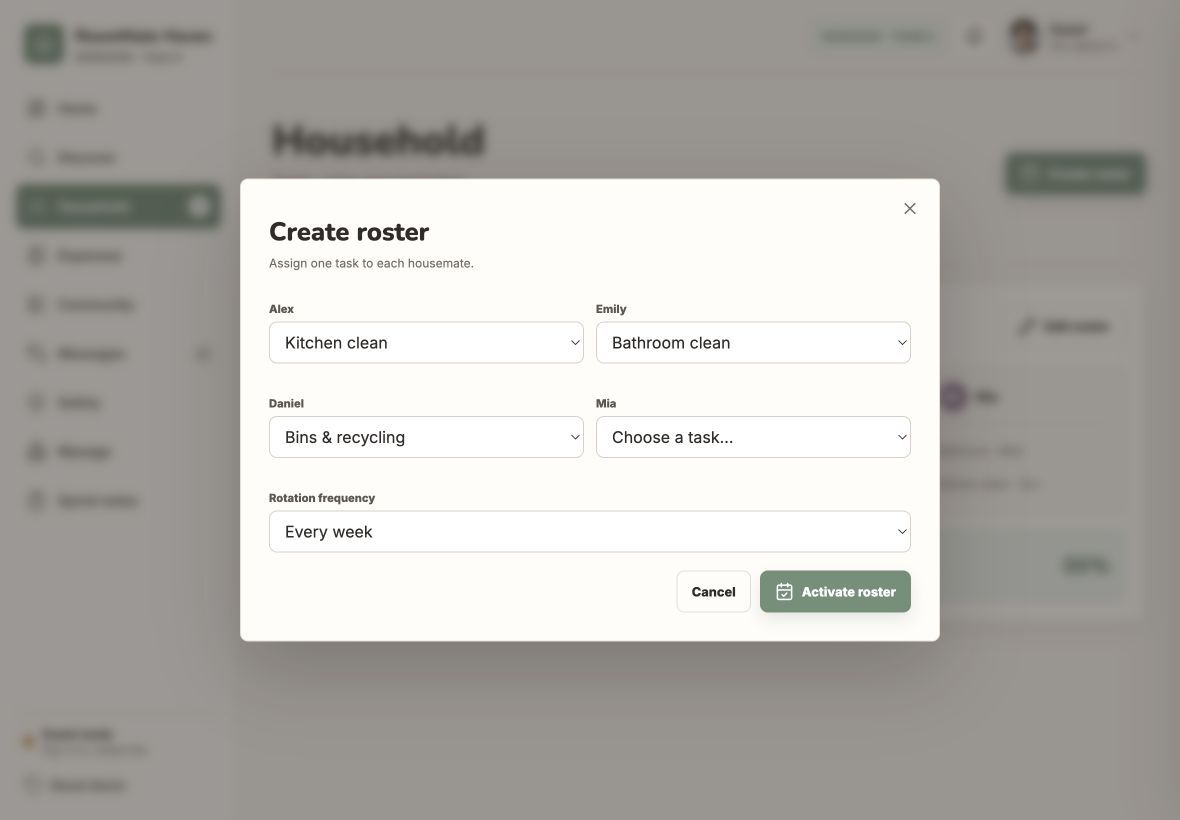
\includegraphics[
            width=\linewidth,
            height=0.18\textheight,
            keepaspectratio
        ]{tests/UserA-T5-roster-modal-focus.png}
        \caption{User A/T5: roster-dialog state. Focus escape, Escape-key
        behaviour and focus return were verified through interaction checks.}
        \label{figuseraevidence}
    \end{subfigure}
    \hfill
    \begin{subfigure}[t]{0.485\textwidth}
        \centering
        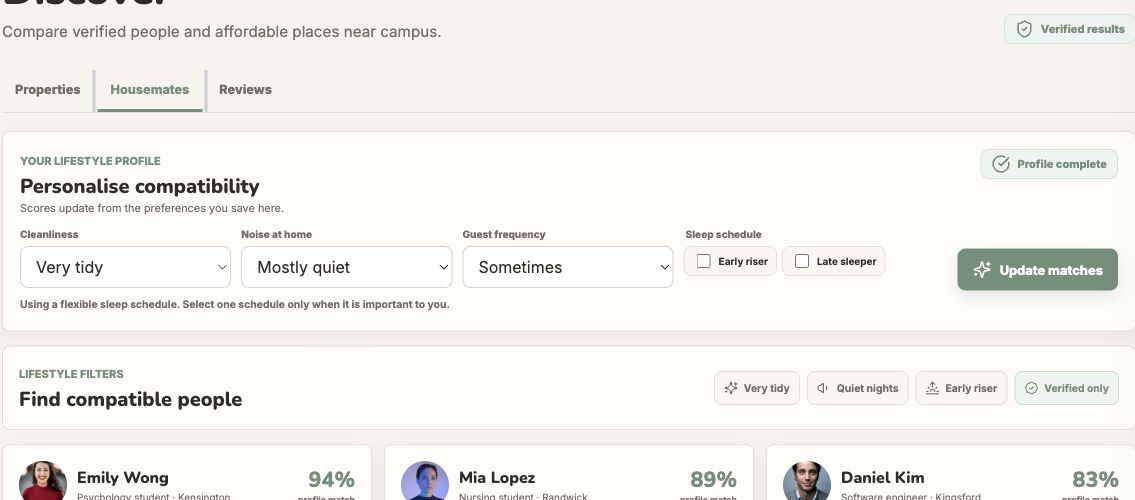
\includegraphics[
            width=\linewidth,
            height=0.18\textheight,
            keepaspectratio
        ]{tests/UserB-T2-tab-keyboard-selected-state.png}
        \caption{User B/T2: Discover selected-state styling. Arrow-key
        behaviour was verified through an interaction check.}
        \label{figuserbevidence}
    \end{subfigure}

    \vspace{0.45em}

    \begin{subfigure}[t]{0.485\textwidth}
        \centering
        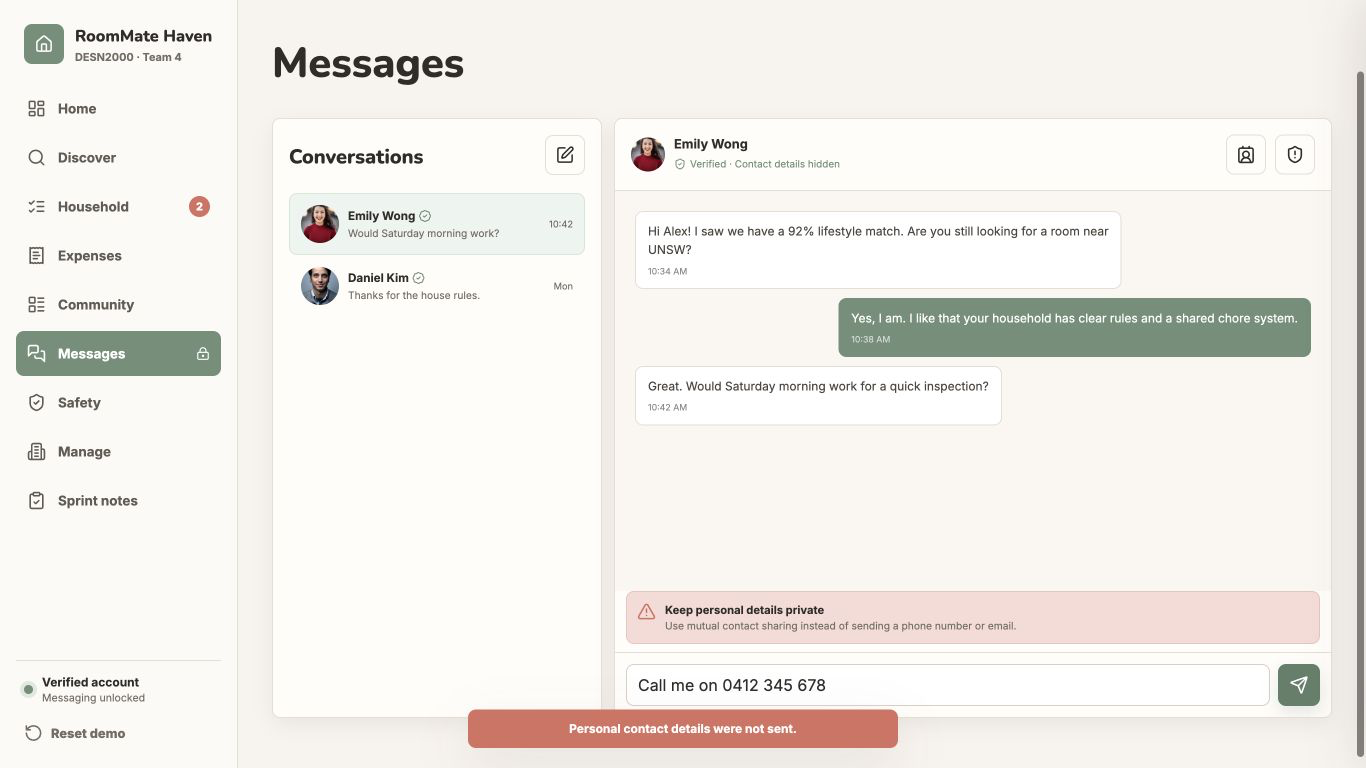
\includegraphics[
            width=\linewidth,
            height=0.18\textheight,
            keepaspectratio
        ]{tests/UserC-T4-contact-block-clarity.png}
        \caption{User C/T4: blocked contact details, privacy warning and the
        separate icon-only contact-sharing control.}
        \label{figuserct4evidence}
    \end{subfigure}
    \hfill
    \begin{subfigure}[t]{0.485\textwidth}
        \centering
        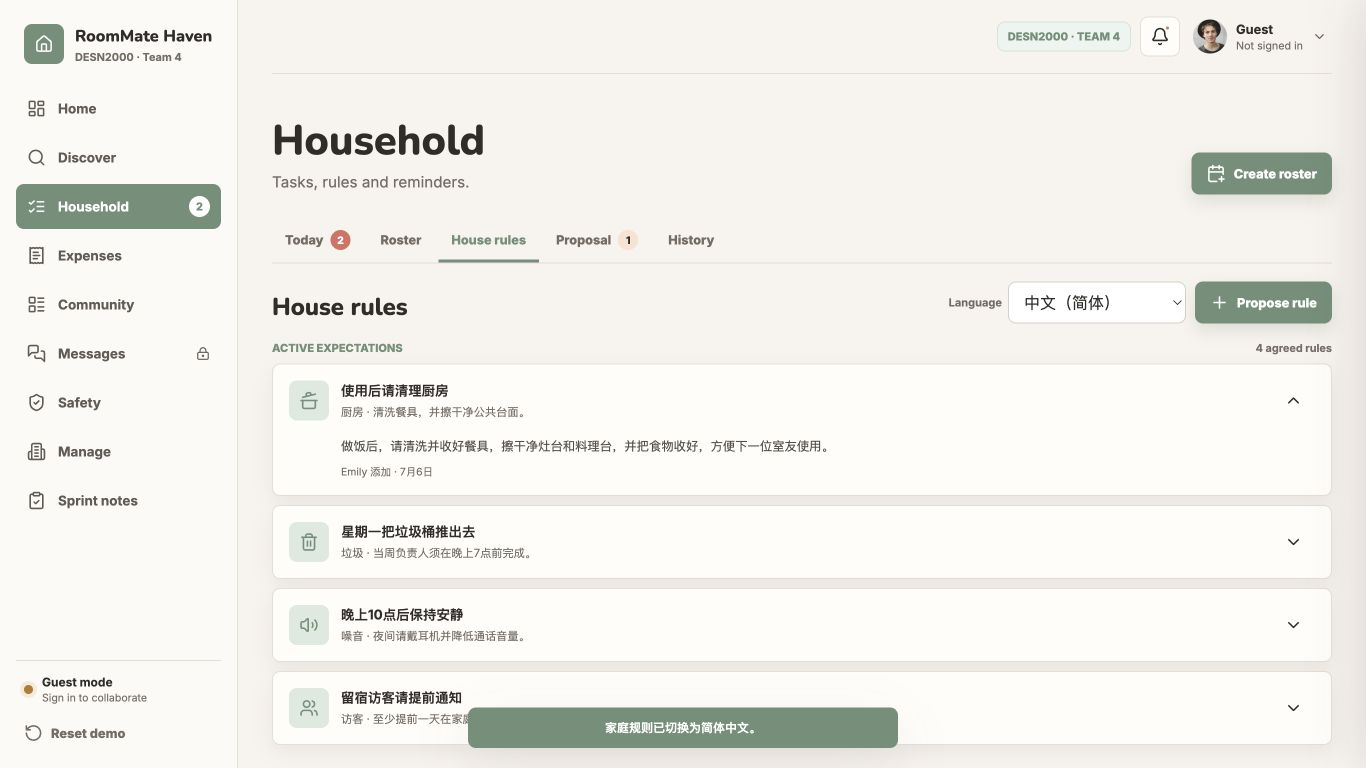
\includegraphics[
            width=\linewidth,
            height=0.18\textheight,
            keepaspectratio
        ]{tests/UserC-T5-mixed-language.png}
        \caption{User C/T5: translated rule content surrounded by English
        headings, labels and actions.}
        \label{figuserct5evidence}
    \end{subfigure}
    \caption{Tablet and laptop evidence for the participant-level findings in
    Table~\ref{tabparticipantfindings}.}
    \label{figparticipantdesktop}
\end{figure}

\begin{figure}[H]
    \centering
    \begin{subfigure}[t]{0.31\textwidth}
        \centering
        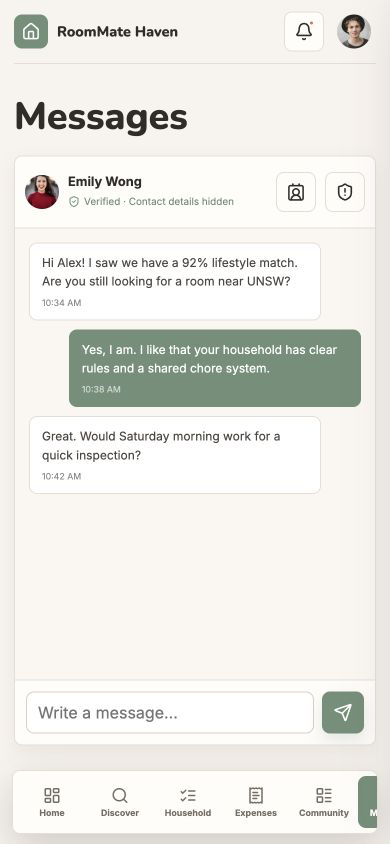
\includegraphics[
            width=\linewidth,
            height=0.31\textheight,
            keepaspectratio
        ]{tests/UserD-T4-mobile-conversation-controls.png}
        \caption{User D/T4: mobile message view without a visible conversation
        switcher or New message control.}
        \label{figuserdevidence}
    \end{subfigure}
    \hfill
    \begin{subfigure}[t]{0.31\textwidth}
        \centering
        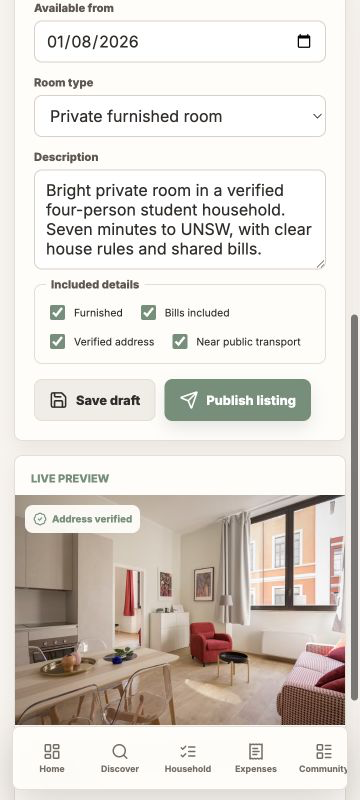
\includegraphics[
            width=\linewidth,
            height=0.31\textheight,
            keepaspectratio
        ]{tests/UserE-T5-save-draft-no-feedback.png}
        \caption{User E/T5: Save draft after activation, with no visible
        confirmation or state change.}
        \label{figuseresaveevidence}
    \end{subfigure}
    \hfill
    \begin{subfigure}[t]{0.31\textwidth}
        \centering
        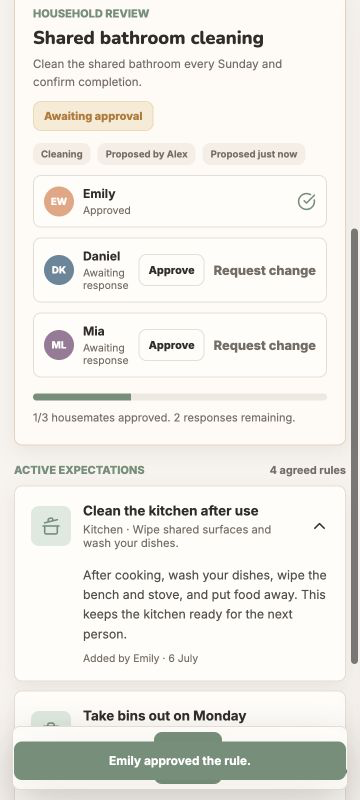
\includegraphics[
            width=\linewidth,
            height=0.31\textheight,
            keepaspectratio
        ]{tests/UserE-T5-mobile-approval-status.png}
        \caption{User E/T5: one-of-three approval state and the separate
        activation-status information.}
        \label{figusereapprovalevidence}
    \end{subfigure}
    \caption{Mobile evidence for the participant-level findings in
    Table~\ref{tabparticipantfindings}.}
    \label{figparticipantmobile}
\end{figure}

Figure~\ref{figbaselinesevidence} consolidates the original task-level
post-session recreations
captured from the same Sprint 1 HTML build at a 1440 by 900 viewport using local
Playwright on 27 July 2026. They document the interface states before Iteration
2 refinement, rather than participant behaviour; the behavioural evidence is
reported in Table~\ref{tabiterationoneoutcomes}.

\begin{figure}[H]
    \centering
    \begin{subfigure}[t]{0.485\textwidth}
        \centering
        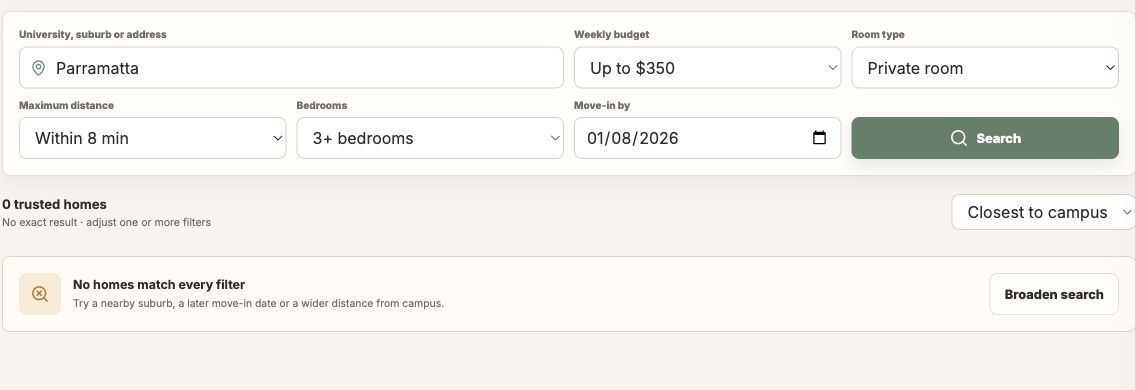
\includegraphics[
            width=\linewidth,
            height=0.18\textheight,
            keepaspectratio
        ]{evidence/sprint1-t1-empty-results-evidence.png}
        \caption{T1, AC-US13-04: the secondary ``Broaden search'' action
        supported a more prominent reset action.}
        \label{figt1evidence}
    \end{subfigure}
    \hfill
    \begin{subfigure}[t]{0.485\textwidth}
        \centering
        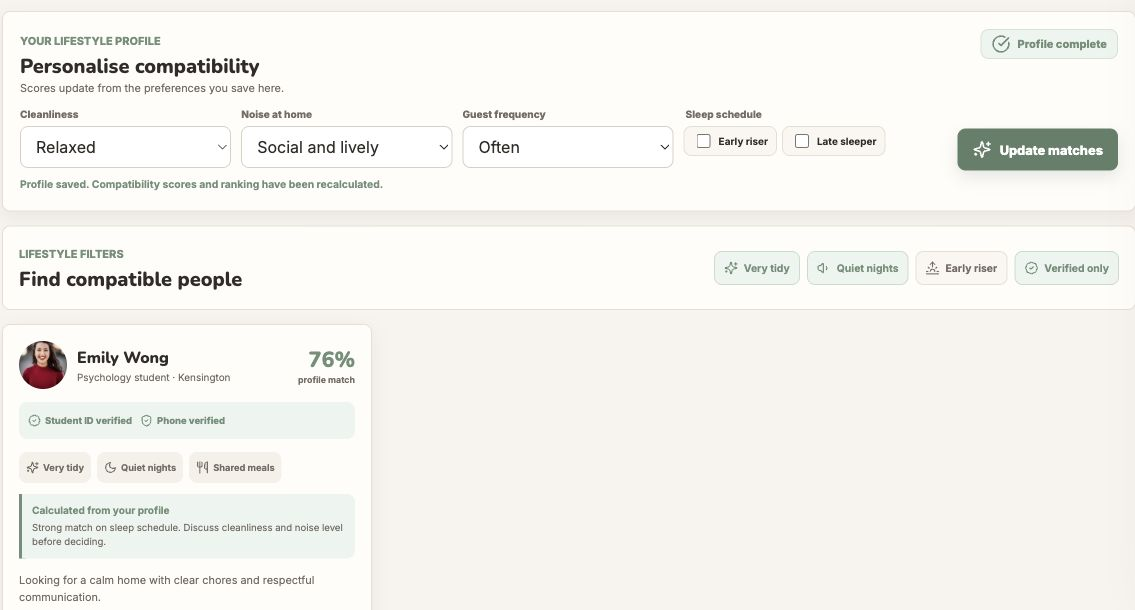
\includegraphics[
            width=\linewidth,
            height=0.18\textheight,
            keepaspectratio
        ]{evidence/sprint1-t2-t3-badges-score-evidence.png}
        \caption{T2--T3, AC-US11-02 and AC-US12-02: small trust and score
        explanations supported larger text and non-colour cues.}
        \label{figt2t3evidence}
    \end{subfigure}

    \vspace{0.45em}

    \begin{subfigure}[t]{0.485\textwidth}
        \centering
        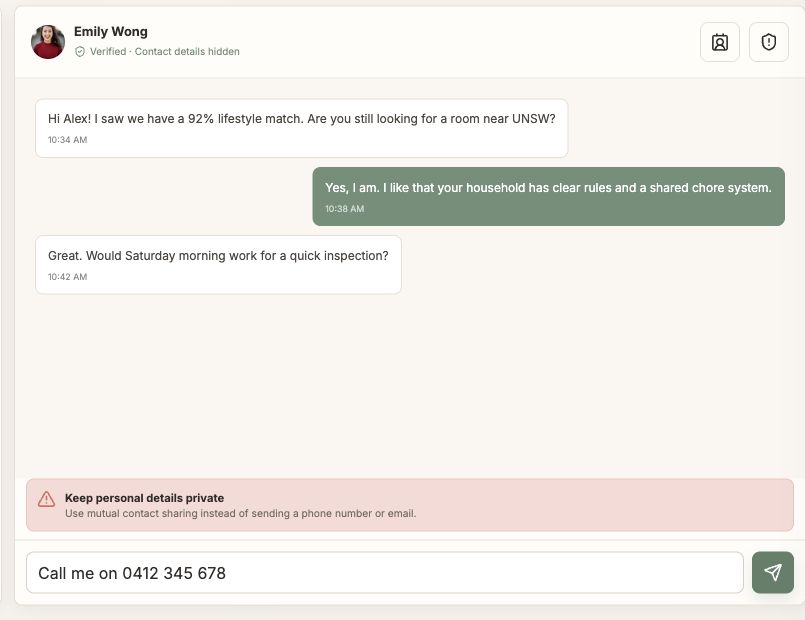
\includegraphics[
            width=\linewidth,
            height=0.18\textheight,
            keepaspectratio
        ]{evidence/sprint1-t4-contact-block-evidence.png}
        \caption{T4, AC-US09-04: the warning and icon-only sharing control were
        separated, making the next step less apparent.}
        \label{figt4evidence}
    \end{subfigure}
    \hfill
    \begin{subfigure}[t]{0.485\textwidth}
        \centering
        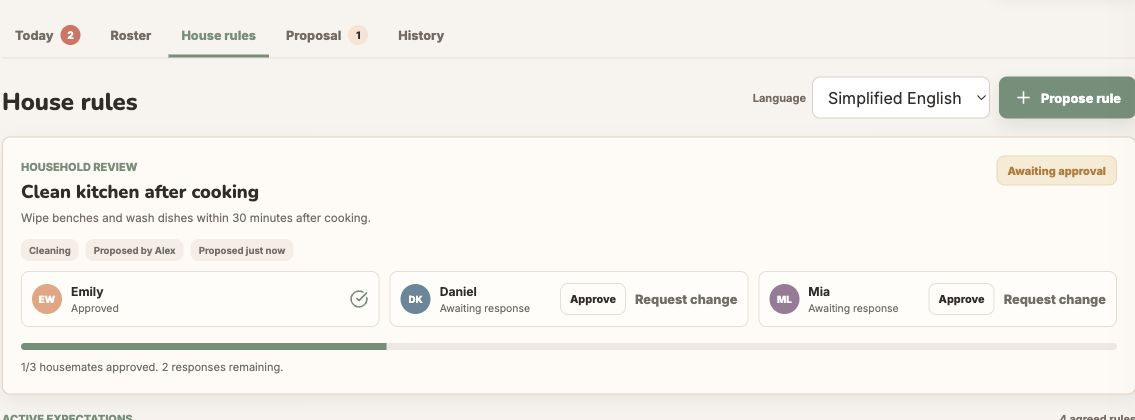
\includegraphics[
            width=\linewidth,
            height=0.18\textheight,
            keepaspectratio
        ]{evidence/sprint1-t5-rule-approval-evidence.png}
        \caption{T5, AC-US10-02: separated approval and activation indicators
        supported a stronger combined status message.}
        \label{figt5evidence}
    \end{subfigure}
    \caption{Compact Sprint 1 task-level baseline evidence before Iteration 2
    refinement.}
    \label{figbaselinesevidence}
\end{figure}

\subsection{Changes after Sprint 1}
\label{subsecchangesaftersprintone}

The team changed states that failed, remained partial or blocked keyboard and
mobile use in Iteration 1. Table~\ref{tabiterationtwochanges} links each design
change to its evidence and revised Jira issue. The Jira cells remain blank
until the revised issues are published.

{\footnotesize
\begin{longtable}{@{}L{0.8cm}L{8.1cm}L{2.5cm}L{2.2cm}@{}}
    \caption{Design changes made after Sprint 1.}
    \label{tabiterationtwochanges}\\
    \toprule
    Task & Design modification & Evidence & Updated Jira link\\
    \midrule
    \endfirsthead
    \caption[]{Design changes made after Sprint 1 continued.}\\
    \toprule
    Task & Design modification & Evidence & Updated Jira link\\
    \midrule
    \endhead
    \midrule
    \multicolumn{4}{r}{Continued on next page}\\
    \endfoot
    \bottomrule
    \endlastfoot

    T1 &
    The empty state places \texttt{Broaden search} beside guidance that
    explains how to recover. &
    Figure~\ref{figiterationtwocore}a &
    \\

    T2 &
    Verification cues pair an icon with readable status text. &
    Figure~\ref{figiterationtwocore}b &
    \\

    T2 &
    Tabs expose their selected state and respond to the arrow, Home and End
    keys. &
    Figure~\ref{figiterationtwotabs} &
    \\

    T3 &
    Each match card explains how the saved profile affected its score and
    names a point to discuss. &
    Figure~\ref{figiterationtwocore}c &
    \\

    T4 &
    The message warning blocks the content, explains mutual sharing and
    announces the result through an alert. &
    Figure~\ref{figiterationtwomessaging}a &
    \\

    T4 &
    The mobile message view keeps a conversation selector and a New
    control. &
    Figure~\ref{figiterationtwomessaging}b &
    \\

    T5 &
    Open dialogs keep keyboard focus, close with Escape and return focus to
    the opening control. &
    Figure~\ref{figiterationtwohousehold}a &
    \\

    T5 &
    Roster validation links the error to the invalid field and moves focus
    to it. &
    Figure~\ref{figiterationtwohousehold}a &
    \\

    T5 &
    Chinese rule content exposes the \texttt{zh-CN} language code to
    assistive technology. &
    Figure~\ref{figiterationtwohousehold}b &
    \\

    T5 &
    Saving a draft updates the page status and shows a confirmation. &
    Figure~\ref{figiterationtwohousehold}c &
    \\
\end{longtable}
}

\subsection{Iteration 2 Test}
\label{subseciterationtwotest}

Iteration 2 used targeted criterion-level retests with the same five
participants after the prototype was revised. Participant observation records
support the reported outcomes; Figures~\ref{figiterationtwocore} to
\ref{figiterationtwohousehold} illustrate the interface states tested but do
not by themselves establish participant performance. Criteria not named in the
retest plan were treated as supplementary regression checks rather than
evidence that an entire multi-criterion task had passed.

\begin{table}[H]
    \centering
    \footnotesize
    \caption{Iteration 2 criterion-level retest plan.}
    \label{tabiterationtwoplan}
    \begin{tabularx}{\textwidth}
        {@{}L{0.7cm}L{2.0cm}L{3.9cm}L{4.2cm}Y@{}}
        \toprule
        Task & Retested AC & Test case & Success threshold &
        Recorded measures\\
        \midrule

        T1 &
        AC-US13-04 &
        Starting from a no-results state, independently change the search
        so that at least one valid result is displayed. &
        At least 4/5 participants recover independently within 60 seconds,
        without a facilitator prompt. &
        Completion time, errors, assistance and interpretation of the
        recovery guidance.\\

        T3 &
        AC-US12-02 &
        Inspect a compatibility result and explain where its score comes
        from and what the score cannot establish. &
        At least 4/5 correctly identify its preference-based evidence and
        do not interpret it as an identity or safety guarantee. &
        Explanation accuracy, completion time and assistance.\\

        T4 &
        AC-US09-04 &
        Attempt to send a message containing personal contact details, then
        explain whether the details were sent and identify the safe next step. &
        At least 4/5 independently confirm that the details remain unsent and
        correctly explain the mutual-sharing condition and next action. &
        Completion, explanation accuracy, errors and assistance.\\

        T5 &
        AC-US10-02 &
        Inspect a proposed rule and determine its approval progress and the
        condition under which it can become active. &
        At least 4/5 correctly explain whether approval is complete and when
        activation can occur. &
        Completion, interpretation accuracy, errors and assistance.\\

        \bottomrule
    \end{tabularx}
\end{table}

\begin{figure}[H]
    \centering
    \begin{subfigure}[t]{0.31\textwidth}
        \centering
        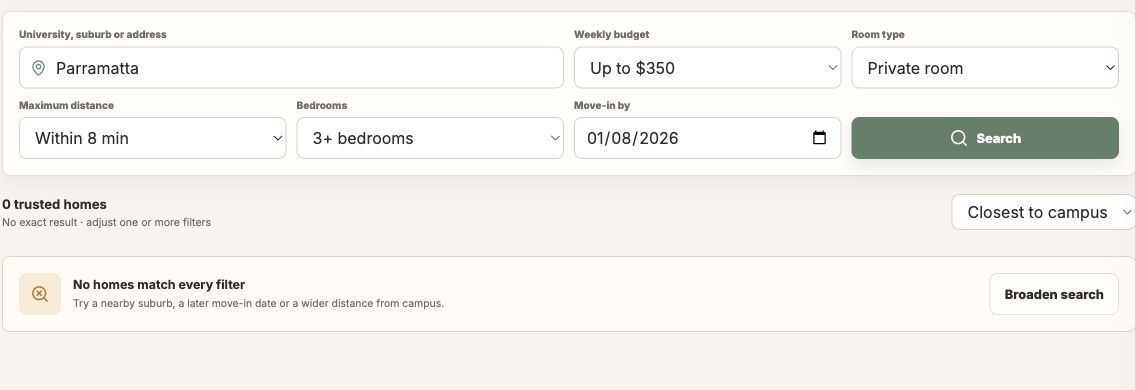
\includegraphics[
            width=\linewidth,
            height=0.17\textheight,
            keepaspectratio
        ]{tests/T1-empty-search-recovery.png}
        \caption{T1 shows recovery guidance beside the empty result.}
    \end{subfigure}
    \hfill
    \begin{subfigure}[t]{0.31\textwidth}
        \centering
        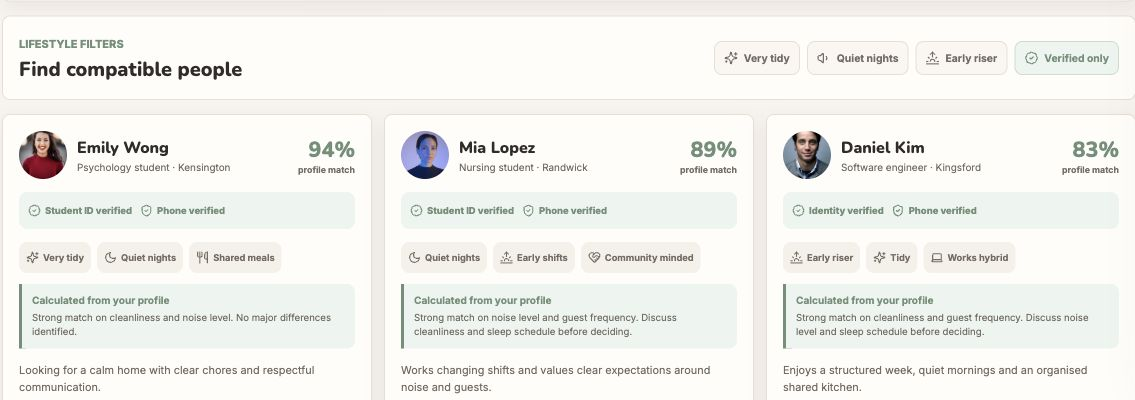
\includegraphics[
            width=\linewidth,
            height=0.17\textheight,
            keepaspectratio
        ]{tests/T2-verification-badge-accessibility.png}
        \caption{T2 shows text and icons for verification.}
    \end{subfigure}
    \hfill
    \begin{subfigure}[t]{0.31\textwidth}
        \centering
        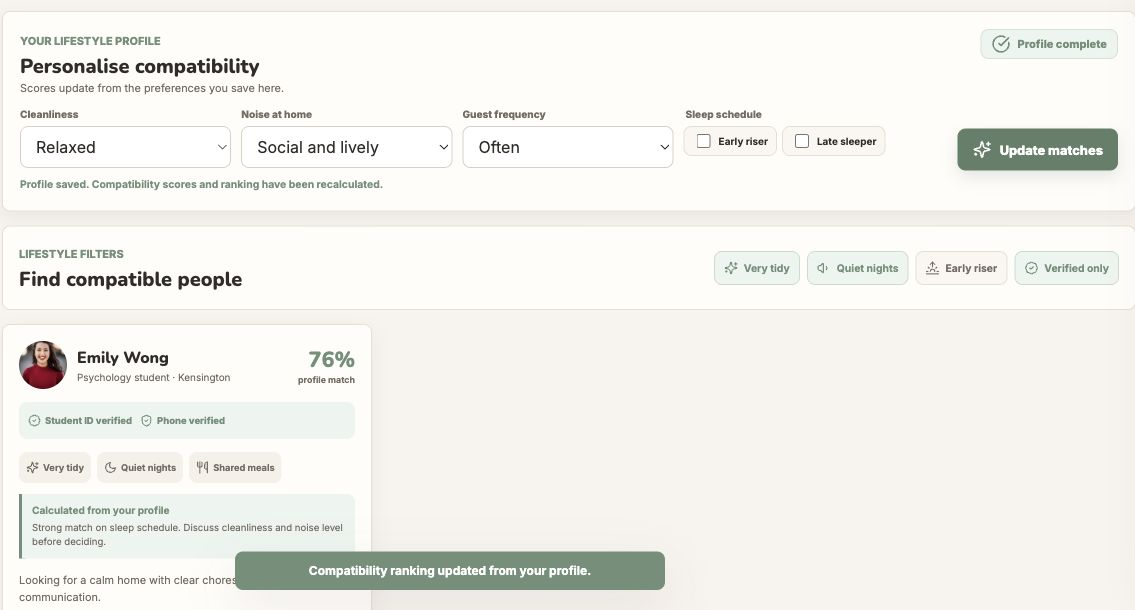
\includegraphics[
            width=\linewidth,
            height=0.17\textheight,
            keepaspectratio
        ]{tests/T3-compatibility-score-explanation.png}
        \caption{T3 explains how the saved profile changed each score.}
    \end{subfigure}
    \caption{Iteration 2 implementation evidence for T1 to T3.}
    \label{figiterationtwocore}
\end{figure}

\begin{figure}[H]
    \centering
    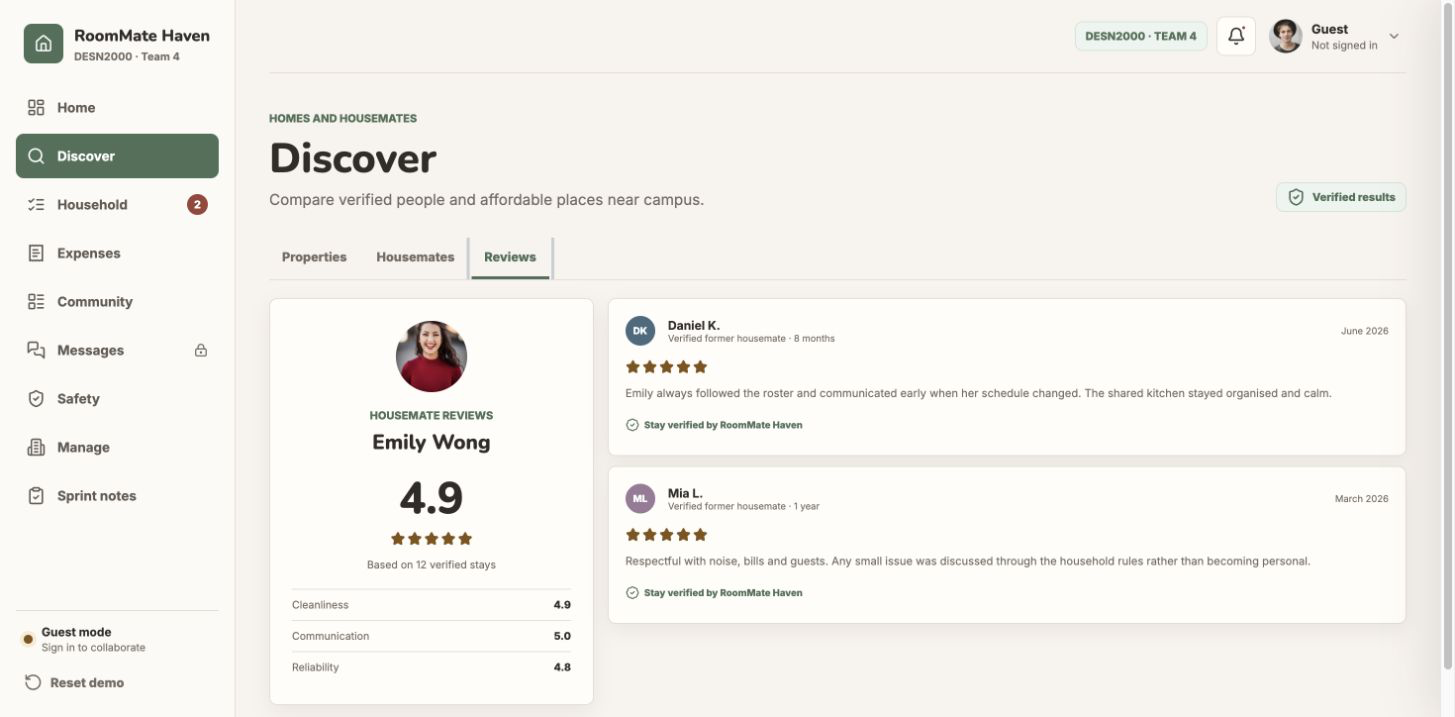
\includegraphics[
        width=0.78\textwidth,
        height=0.30\textheight,
        keepaspectratio
    ]{tests/ITER2-T2-discover-keyboard-tabs.png}
    \caption{T2 tab focus and selected state after keyboard navigation.}
    \label{figiterationtwotabs}
\end{figure}

\begin{figure}[H]
    \centering
    \begin{subfigure}[t]{0.65\textwidth}
        \centering
        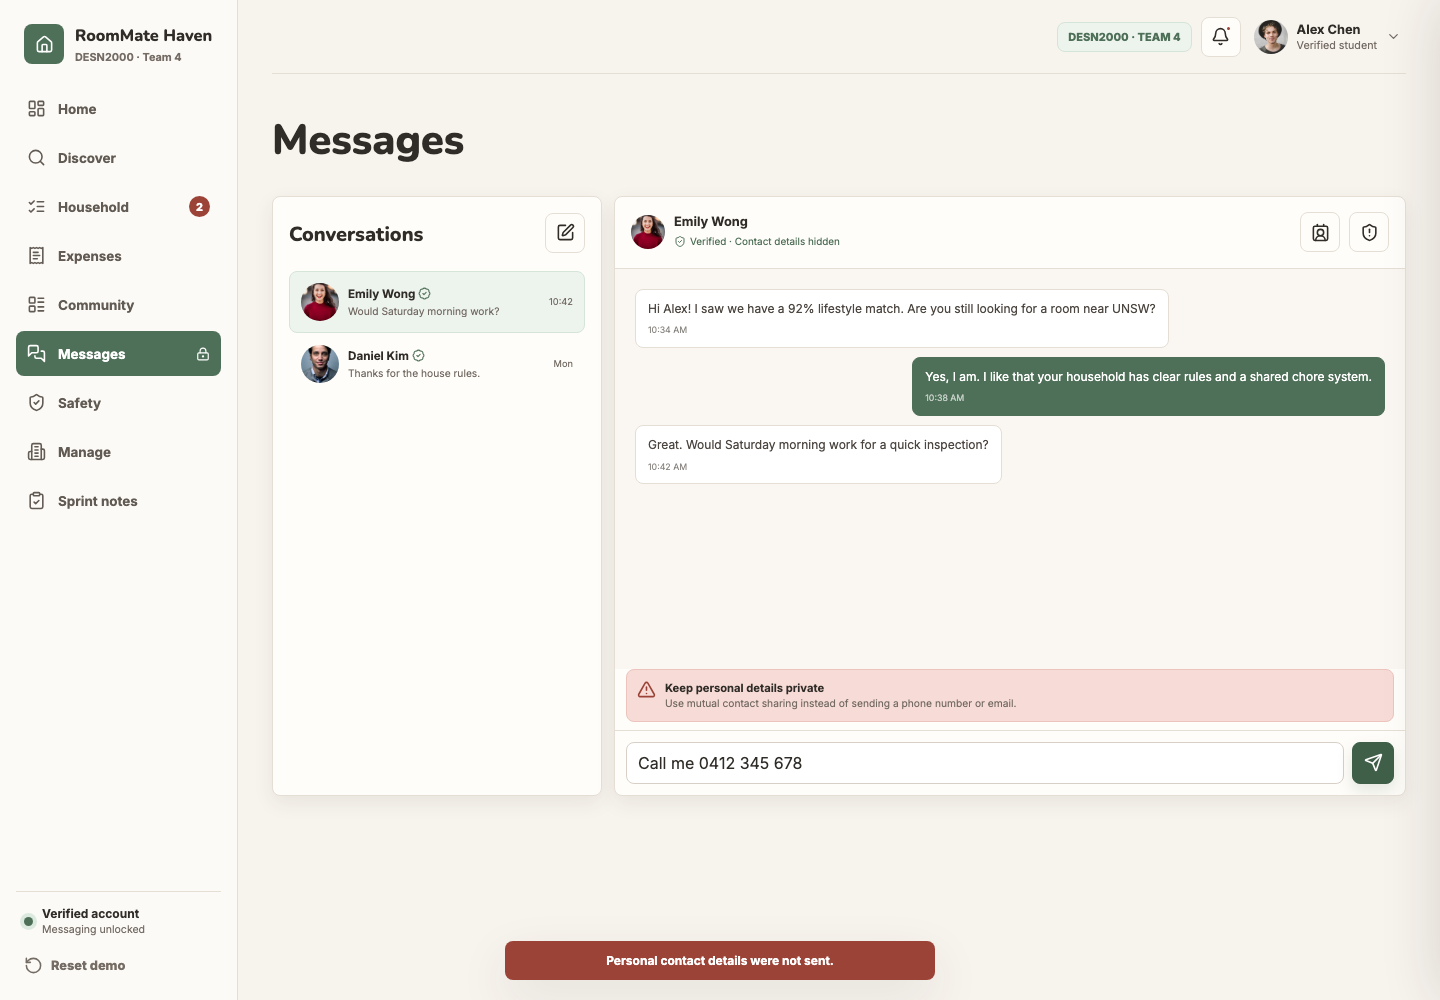
\includegraphics[
            width=\linewidth,
            height=0.28\textheight,
            keepaspectratio
        ]{tests/FIX-06-message-warning-live-alert.png}
        \caption{T4 blocks a phone number and shows the safer next step.}
    \end{subfigure}
    \hfill
    \begin{subfigure}[t]{0.28\textwidth}
        \centering
        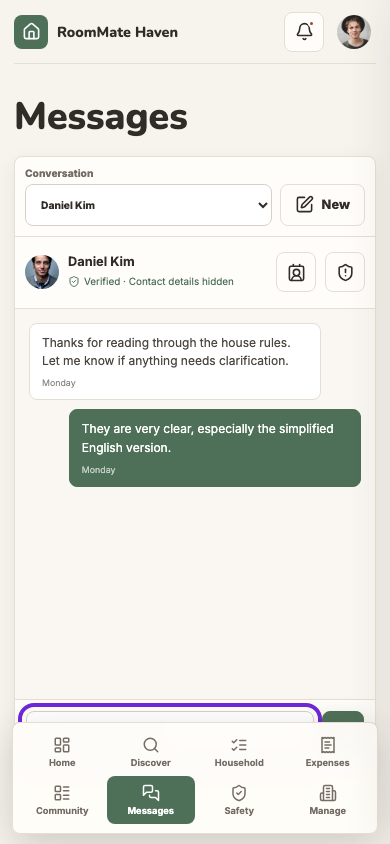
\includegraphics[
            width=\linewidth,
            height=0.28\textheight,
            keepaspectratio
        ]{tests/FIX-08-mobile-conversation-switcher.png}
        \caption{T4 keeps conversation controls at the mobile viewport.}
    \end{subfigure}
    \caption{Iteration 2 implementation evidence for T4.}
    \label{figiterationtwomessaging}
\end{figure}

\begin{figure}[H]
    \centering
    \begin{subfigure}[t]{0.485\textwidth}
        \centering
        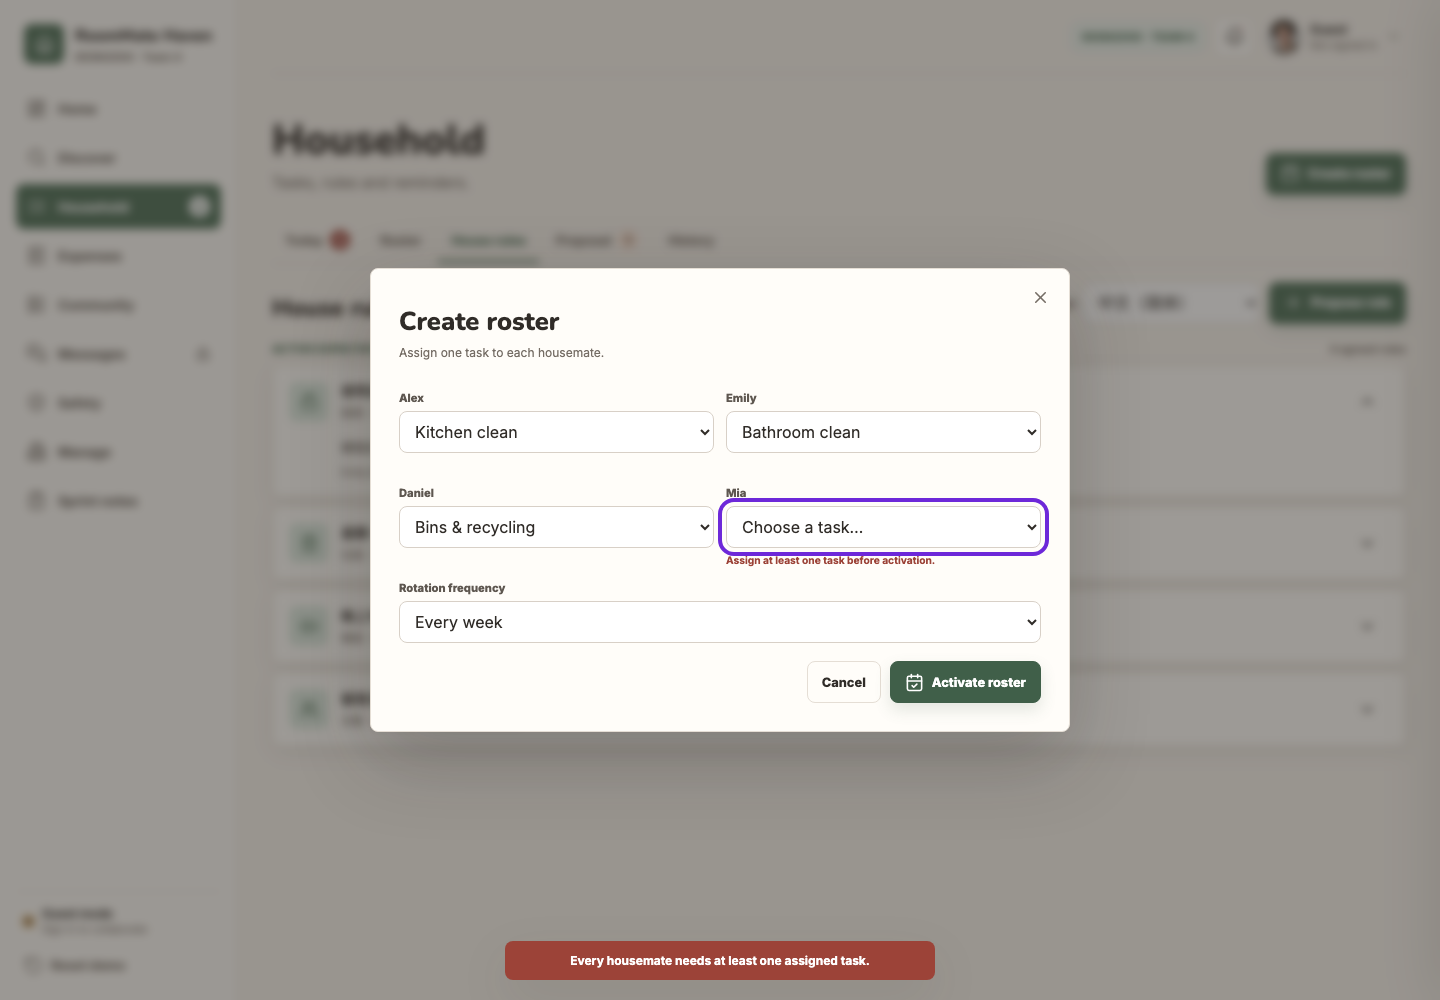
\includegraphics[
            width=\linewidth,
            height=0.22\textheight,
            keepaspectratio
        ]{tests/FIX-13-roster-error-focus.png}
        \caption{T5 keeps focus on the invalid roster field.}
    \end{subfigure}
    \hfill
    \begin{subfigure}[t]{0.485\textwidth}
        \centering
        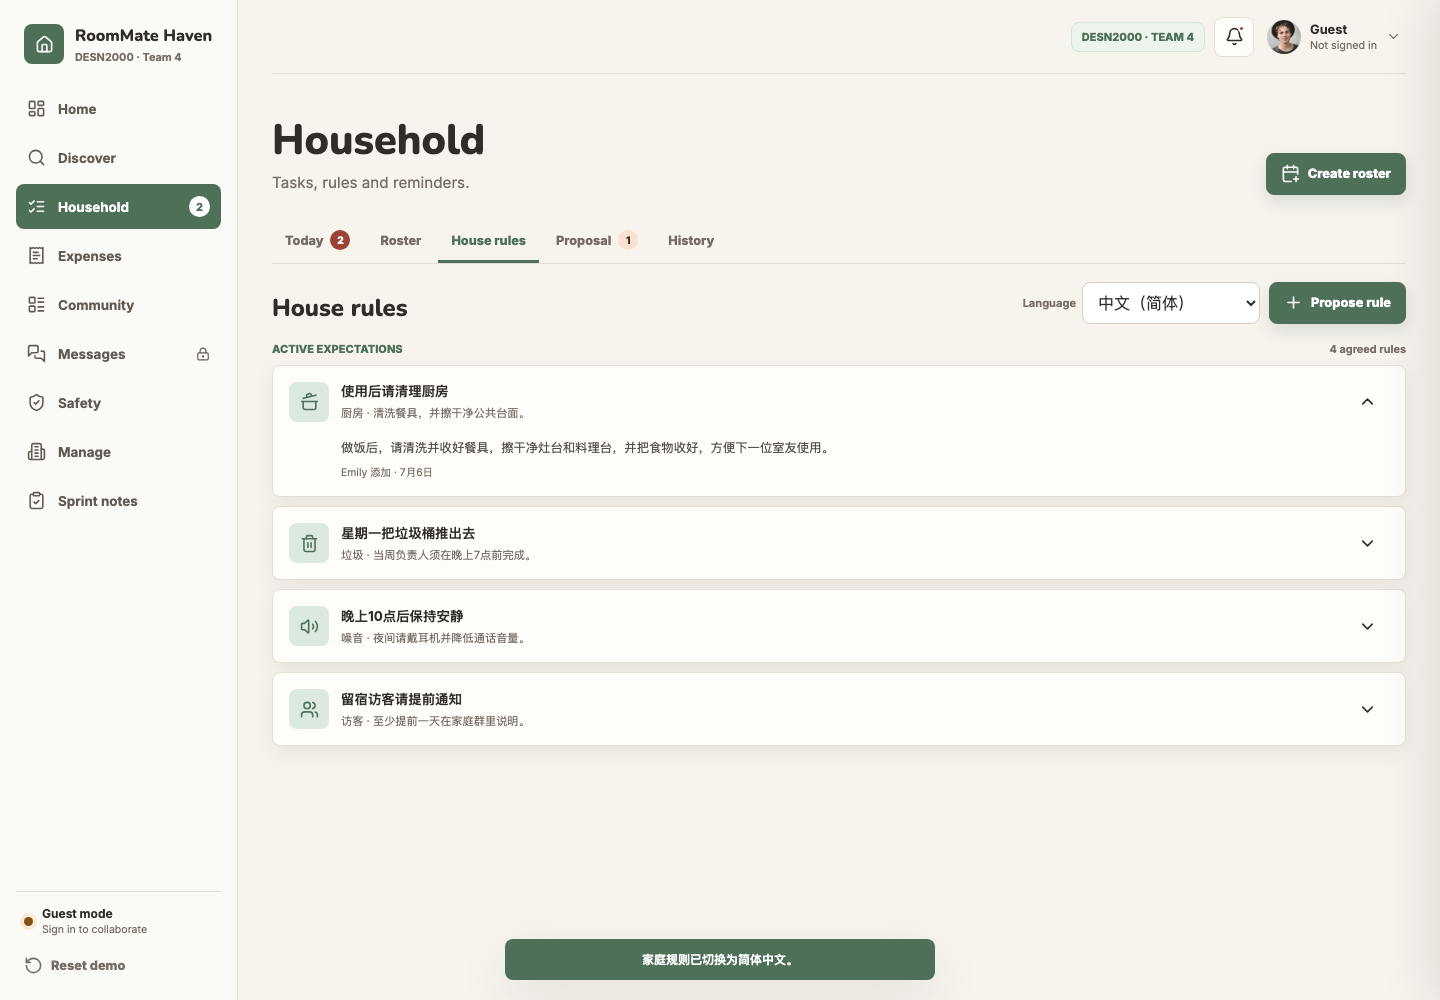
\includegraphics[
            width=\linewidth,
            height=0.22\textheight,
            keepaspectratio
        ]{tests/FIX-12-chinese-language-metadata.png}
        \caption{T5 displays Chinese rules with matching language metadata.}
    \end{subfigure}

    \vspace{0.45em}

    \begin{subfigure}[t]{0.485\textwidth}
        \centering
        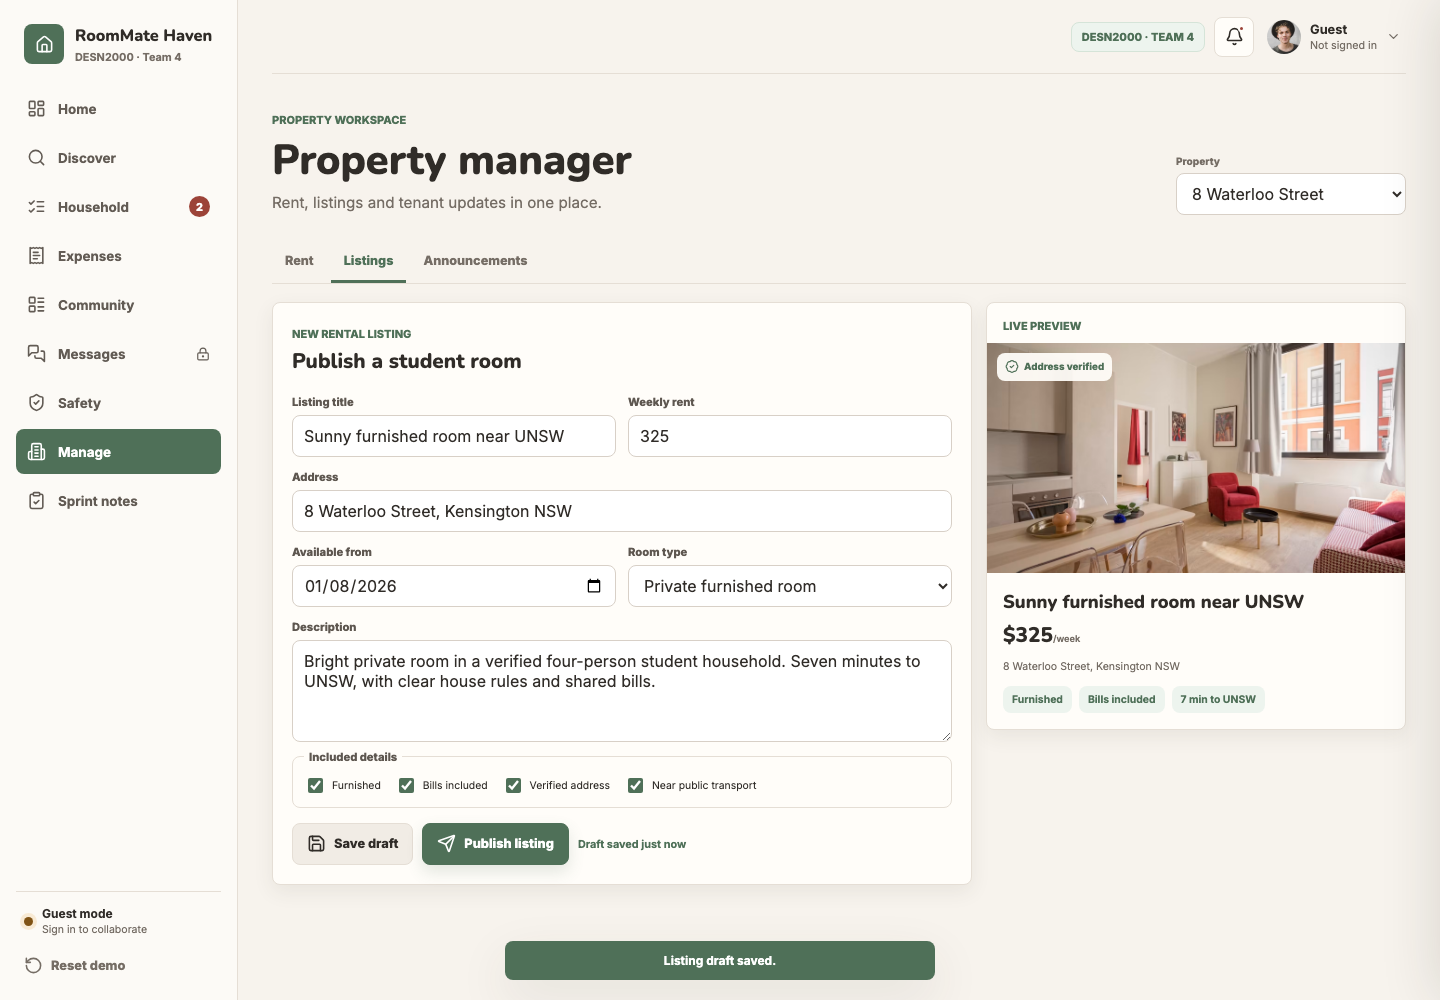
\includegraphics[
            width=\linewidth,
            height=0.22\textheight,
            keepaspectratio
        ]{tests/FIX-10-listing-draft-saved.png}
        \caption{The supplementary draft check shows a saved state.}
    \end{subfigure}
    \hfill
    \begin{subfigure}[t]{0.485\textwidth}
        \centering
        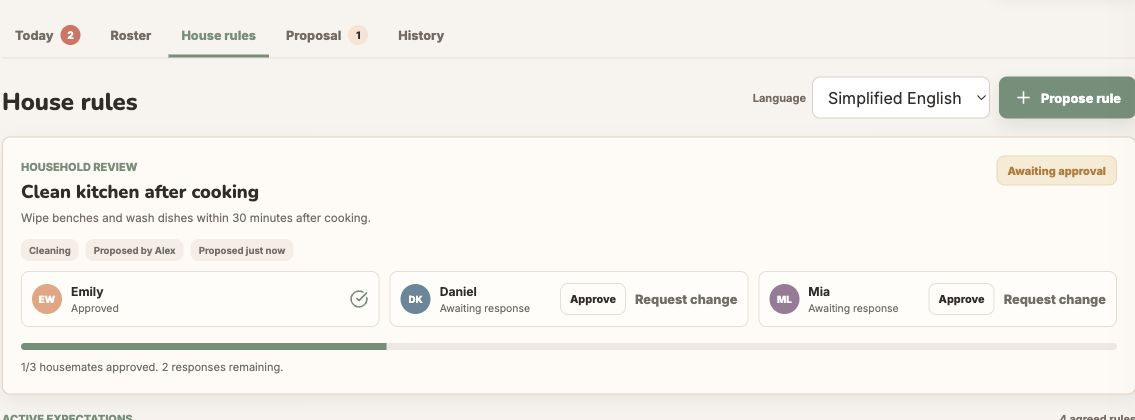
\includegraphics[
            width=\linewidth,
            height=0.22\textheight,
            keepaspectratio
        ]{tests/T5-rule-approval-status.png}
        \caption{T5 still separates progress from the activation condition.}
    \end{subfigure}
    \caption{Iteration 2 implementation evidence for T5 and its remaining
    issue.}
    \label{figiterationtwohousehold}
\end{figure}

\begin{table}[H]
    \centering
    \footnotesize
    \caption{Iteration 2 criterion-level retest results.}
    \label{tabiterationtworetestresults}
    \begin{tabularx}{\textwidth}
        {@{}L{0.7cm}L{1.4cm}L{1.2cm}L{1.8cm}L{0.8cm}YL{1.1cm}@{}}
        \toprule
        Task &
        Independent &
        Assisted &
        Time &
        Errors &
        Interpretation result &
        AC status\\
        \midrule

        T1 &
        4/5 &
        1/5 &
        44 seconds (median) &
        3 &
        4/5 understood how to broaden the search and recover from the
        no-results state. &
        Pass\\

        T3 &
        3/5 &
        2/5 &
        75 seconds (median) &
        2 &
        2/5 correctly explained the preference-based score without treating
        it as evidence of personal safety. &
        Partial\textsuperscript{*}\\

        \bottomrule
    \end{tabularx}

    \vspace{0.3em}
    \begin{minipage}{\textwidth}
        \footnotesize
        \textit{\textsuperscript{*}Partial indicates that the revised
        interface produced observable improvement but did not meet the
        predefined threshold of four successful participants.}
    \end{minipage}
\end{table}

\begin{table}[H]
    \centering
    \footnotesize
    \caption{Iteration 2 results for the modified Sprint 1 tasks.}
    \label{tabiterationtworesults}
    \begin{tabularx}{\textwidth}{@{}L{0.7cm}L{3.8cm}L{3.0cm}L{1.2cm}Y@{}}
    \toprule
    Task & Retest outcome and resolved problem & Acceptance criteria result & New issue & Remaining problem\\
    \midrule

    T1 &
    Completed for the targeted criterion. The empty result gives a recovery
    action and names the inputs that can change. &
    AC-US13-04 changed from Fail to Pass. Other T1 criteria were not separately
    retested. &
    No. &
    None shown.\\

    T2 &
    Supplementary regression check. Text supports each verification cue.
    Keyboard users can identify and change tabs. &
    AC-US11-02 remained Pass from Iteration 1; no other T2 criterion was
    separately retested. &
    No. &
    Participants still confused profile identity verification with the phone
    check that unlocks messaging.\\

    T3 &
    Partially completed for the targeted criterion. The match card explains
    the score source and identifies points to discuss. &
    AC-US12-02 remained Partial because several participants still treated the
    score as a safety signal. Other T3 criteria were not separately retested. &
    No. &
    The score source is visible, but its limit remains unclear.\\

    T4 &
    Completed for the targeted criterion. Contact details remain unsent. The
    warning explains mutual sharing and the mobile view retains both
    conversation actions. &
    AC-US09-04 changed from Fail to Pass. Other T4 criteria were not separately
    retested. &
    No. &
    The desktop sharing action still relies on an icon, so its purpose is less
    clear without hover.\\

    T5 &
    Partially completed for the targeted criterion. Dialog focus, roster
    errors, rule language metadata and draft feedback expose a clear state. &
    AC-US02-02 remained Pass from Iteration 1. AC-US10-02 remained Fail.
    Other T5 criteria were supplementary checks or were not separately
    retested. &
    No. &
    The status still does not explain activation. The Household entry and
    House rules destination use different labels. Surrounding controls remain
    in English after Chinese is selected.\\
    \bottomrule
    \end{tabularx}
\end{table}

\subsection{Persistent Issues and Impact}
\label{subsecpersistentissues}

The same five participants tested both iterations. Several still struggled to
explain what the compatibility score measured after the second test. Although
the revised cards linked the score to saved preferences, some users treated a
high score as evidence that a person was safe. This could cause them to
misjudge a potential housemate.

Confusion also persisted between a verified profile and phone verification.
Similar visual cues made the two states appear equivalent, even though identity
verification supports profile trust and phone verification only unlocks
messaging. The ambiguity increased decision time and weakened confidence in
the safety process.

Navigation remained unclear because the main entry was named Household while
the destination was named House rules. Users opened the wrong view before
finding rule proposals. They also struggled in both rounds to connect approval
progress with activation. These problems caused repeated checking and left
users uncertain about which household rules applied.

\end{document}
